%iffalse
\let\negmedspace\undefined
\let\negthickspace\undefined
\documentclass[journal,12pt,onecolumn]{IEEEtran}
\usepackage{cite}
\usepackage{amsmath,amssymb,amsfonts,amsthm}
\usepackage{algorithmic}
\usepackage{graphicx}
\usepackage{textcomp}
\usepackage{xcolor}
\usepackage{txfonts}
\usepackage{listings}
\usepackage{enumitem}
\usepackage{mathtools}
\usepackage{gensymb}
\usepackage{comment}
\usepackage[breaklinks=true]{hyperref}
\usepackage{tkz-euclide} 
\usepackage{listings}
\usepackage{gvv}                                        
%\def\inputGnumericTable{}                                 
\usepackage[latin1]{inputenc}                                
\usepackage{color}                                            
\usepackage{array}                                            
\usepackage{longtable}                                       
\usepackage{calc}                                             
\usepackage{multirow}                                         
\usepackage{hhline}                                           
\usepackage{ifthen}                                           
\usepackage{lscape}
\usepackage{tabularx}
\usepackage{array}
\usepackage{float}
\usepackage{pgfplots}


\newtheorem{theorem}{Theorem}[section]
\newtheorem{problem}{Problem}
\newtheorem{proposition}{Proposition}[section]
\newtheorem{lemma}{Lemma}[section]
\newtheorem{corollary}[theorem]{Corollary}
\newtheorem{example}{Example}[section]
\newtheorem{definition}[problem]{Definition}
\newcommand{\BEQA}{\begin{eqnarray}}
\newcommand{\EEQA}{\end{eqnarray}}
\newcommand{\define}{\stackrel{\triangle}{=}}
\theoremstyle{remark}
\newtheorem{rem}{Remark}

% Marks the beginning of the document
\begin{document}
\bibliographystyle{IEEEtran}
\vspace{3cm}

\title{assignment3:7.3.4}
\author{AI24BTECH11007 - Sri Sathwik Desaboina}
\maketitle
\bigskip

\renewcommand{\thefigure}{\theenumi}
\renewcommand{\thetable}{\theenumi}
\textbf{Question}:\\
Show that the point $\myvec{x \\ y}$ given by $x = \frac{2at}{1 + t^2}$ and $y = \frac{a(1 - t^2)}{1 + t^2}$ lies on a circle for all real values of $t$ such that $-1 \leq t \leq 1$, where $a$ is any given real number.
\\
\textbf{Solution: }
\begin{table}[h!]    
    \centering
    \begin{tabular}[12pt]{ |c| c| c|}
    \hline
    \textbf{S.No} & \textbf{variables used}&\textbf{description}\\ 
    \hline
	$1$ & \textit{t} & a variable which takes the real values in the range $(-1,1)$\\
    \hline
	$2$ & \textit{a} & it is a fixed real number \\
    \hline
	$3$ & $\vec{A(t)}$ & it is a transformation matrix of parameter t\\
    \hline
	$4$ & $\vec{v(t)}$ & it represent the parameter t and allows to define x and y \\
    \hline
	$5$ & $\vec{p(t)}$ & a point with coordinates x and y. \\
    \hline
    \end{tabular}

    \caption{Input parameters }
    \label{table}
  \end{table}

 \begin{align*}
\text{Given } & x = \frac{2at}{1 + t^2}, \quad y = \frac{a(1 - t^2)}{1 + t^2}, \\
\text{let } & \mathbf{p}(t) = \myvec{x \\ y} = \myvec{\frac{2at}{1 + t^2} \\ \frac{a(1 - t^2)}{1 + t^2}}. \\
\text{Expressing } & \mathbf{p}(t) \text{ in matrix form:} \\
 \implies \mathbf{A}(t) & = \begin{pmatrix} \frac{2a}{1+t^2} & 0 \\ 0 & \frac{a(1-t^2)}{1+t^2} \end{pmatrix}, \\
	 \implies \mathbf{v}(t) & = \myvec{t \\ t^2}, \\
 \implies \mathbf{p}(t) & = \begin{pmatrix} \frac{2a}{1+t^2} & 0 \\ \frac{a(1 - t^2)}{1+t^2} & 0 \end{pmatrix} \myvec{t \\ 1}. \\
\text{Then } & x^2 + y^2 = a^2. \\
\text{Thus, } & \mathbf{p}(t)^T \begin{pmatrix} 1 & 0 \\ 0 & 1 \end{pmatrix} \mathbf{p}(t) = a^2.
\end{align*}
$\therefore$ It is proved that the locus of all these points forms a circle.


Plot:
\begin{figure}[h!]
    \centering
	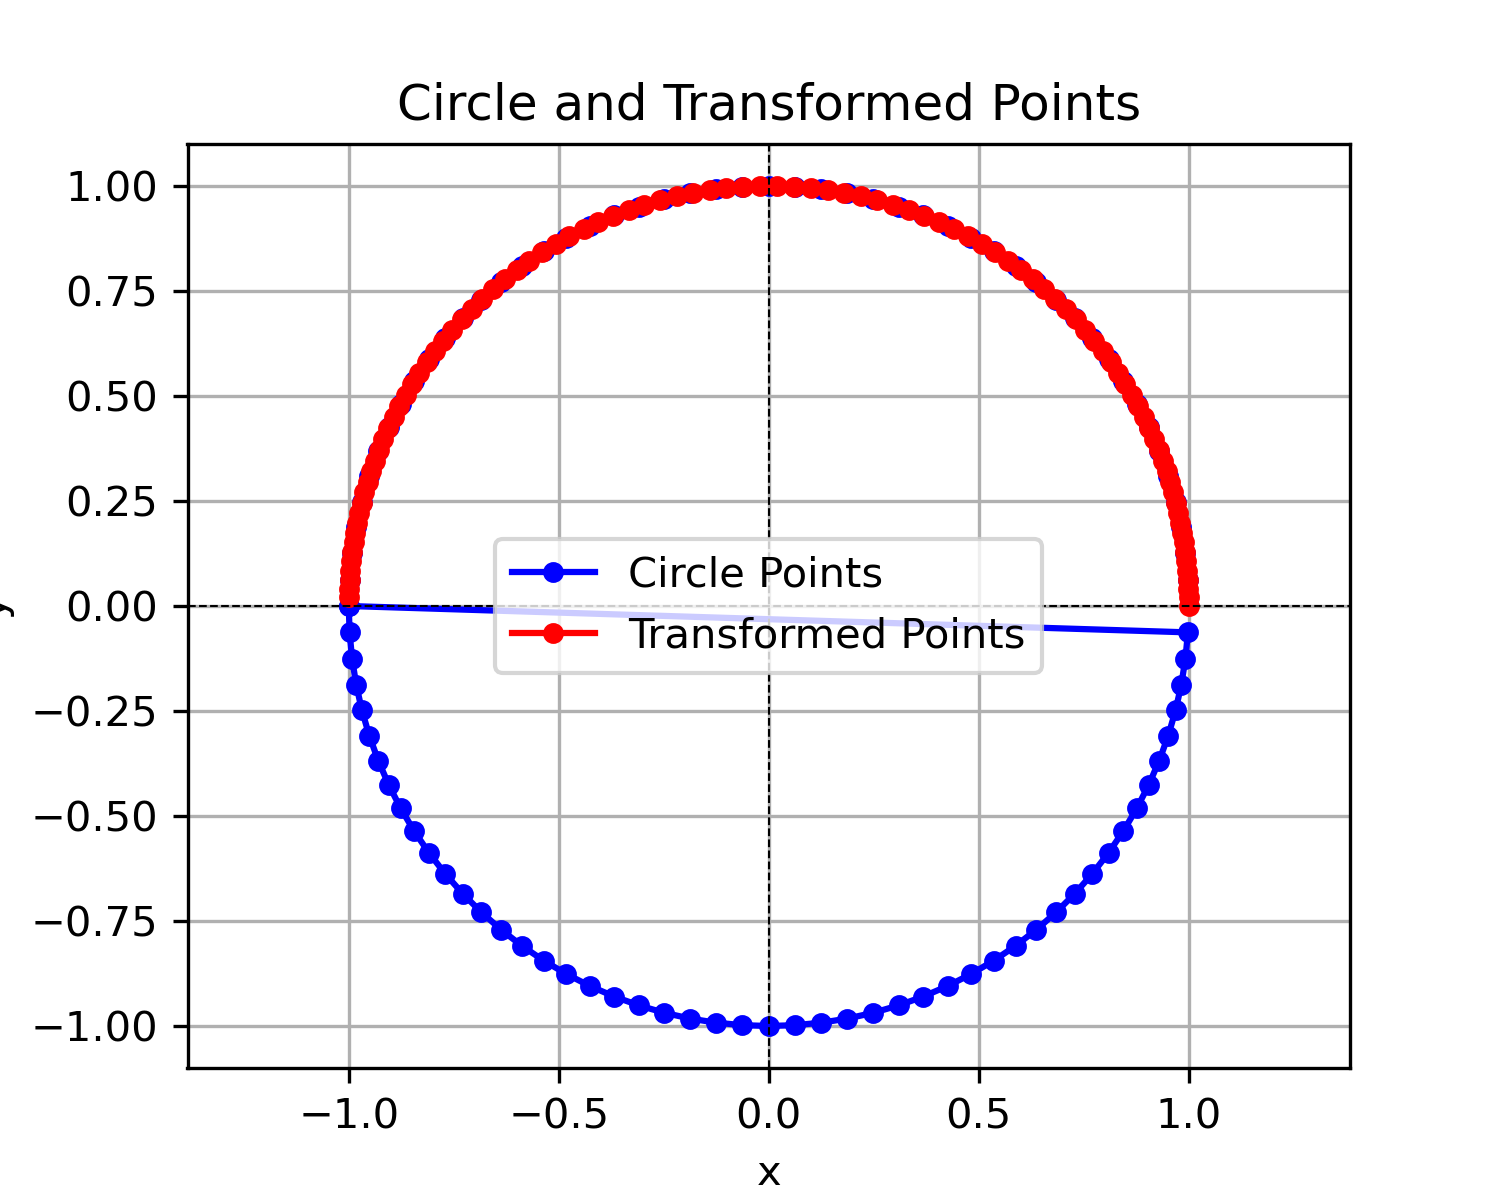
\includegraphics[scale=0.8]{figs/plot.png}
	\caption{Circle with center$\vec{O} \myvec{0\\0}$ and with radius $a=1$ units.} 

    \label{fig:plot}
\end{figure}


\end{document}









